\documentclass[10pt,a4paper]{article}
\usepackage[utf8]{inputenc}
\usepackage[francais]{babel}
\usepackage[T1]{fontenc}
\usepackage{hyperref}
\usepackage{eurosym}
\usepackage{ amssymb }
\usepackage{graphics}
\usepackage{pdfpages}
\usepackage{placeins}
\usepackage{float}

\begin{document}

\begin{titlepage}
    \begin{center}
        \textbf{\textsc{UNIVERSIT\'E LIBRE DE BRUXELLES}}\\
        \vfill{}\vfill{}
        \begin{center}{\Huge Rapport : Annuaire d’établissements horeca}\end{center}{\Huge \par}
        \begin{center}{\large Romain \textsc{Fontaine}, Nikita \textsc{Marchant}}\end{center}{\Huge \par}
        \vfill{}\vfill{} \vfill{}
        \begin{flushleft}{\large \textbf{INFO-H-303 Base de données}}\hfill{Esteban Zimányi, Michaël Waumans}\end{flushleft}{\large\par}
        \vfill{}\vfill{}\enlargethispage{3cm}
        \textbf{Année académique 2015--2016}
    \end{center}
\end{titlepage}

\setlength{\parindent}{1.5em}
\setlength{\parskip}{1em}
\linespread{1.1}

\section{Diagramme entité association}
\subsection{Diagramme}
\begin{figure}[h]
    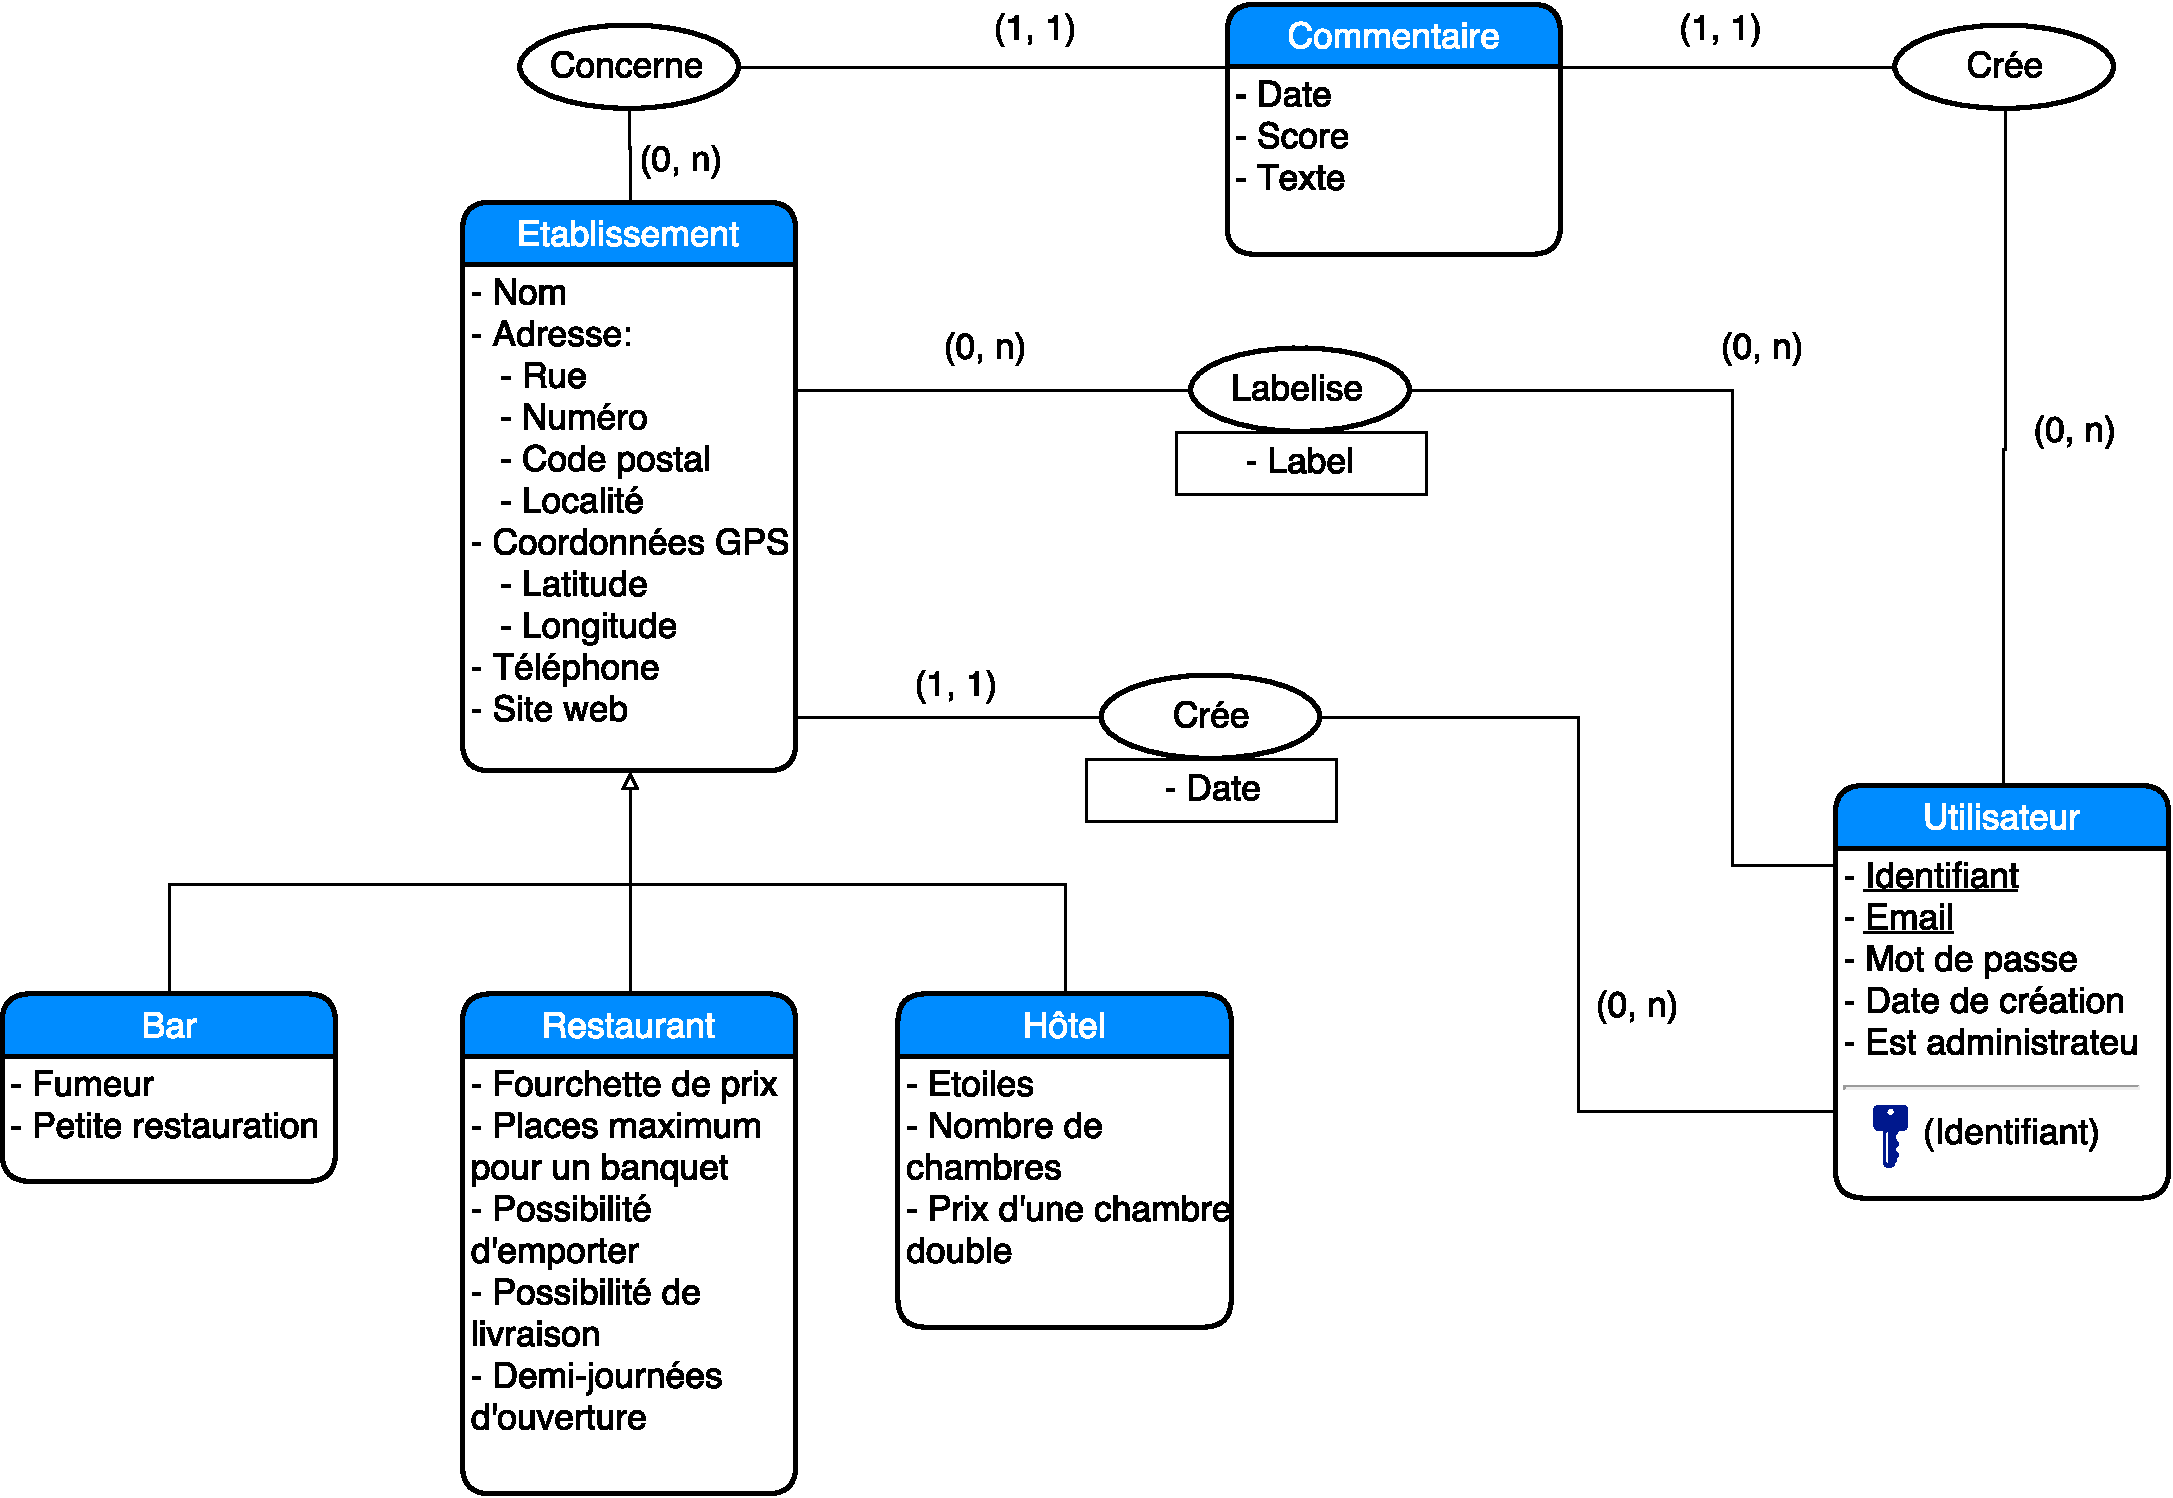
\includegraphics[scale=0.40]{EA.pdf}
    \caption{Diagramme Entité-Association}
    \label{diagram}
\end{figure}
\FloatBarrier

\subsection{Contraintes}

Les contraintes sont les suivantes :
\begin{itemize}
  \item L'\textit{UtilisateurId} d'un \textit{Etablissement} ne peut référencer qu'un \textit{Utilisateur} dont le champ \textit{EstAdministrateur} est vrai.
  \item La \textit{DateCretation} d'un \textit{Etablissement} doit être surpérieure à la \textit{DateCretation} de l'\textit{Utilisateur} qui l'a créé.
  \item La \textit{Latitude} (respectivement \textit{Longitude}) d'un \textit{Etablissement} doit appartenir à l'intervalte $[-90, 90]$ (respectivement $[-180, 180]$)
  \item Le champ \textit{Etoiles} d'un \textit{Hotel} doit appartenir à $[0,5]$
  \item Le champ \textit{Etoiles} d'un \textit{Commentaire} doit appartenir à $[0,5]$

\end{itemize}




\section{Modèle relationnel}
\subsection{Modèle}


\begin{description}
\item[Utilisateur](
    \underline{Id},
    \underline{Email},
    MotDePasse,
    DateCretaion,
    EstAdministrateur)

\item[Etablissement](
    \underline{Id},
    Type,
    Nom,
    Telephone,
    \textit{SiteWeb},
    Rue,
    Numero,
    CodePostal,
    Localite,
    Latitude,
    Longitude,
    DateCretation
    UtilisateurId)

    \begin{itemize}
        \item Etablissement.Type est une énumération de (Hotel, Bar, Restaurant)
        \item Etablissement.UtilisateurId référence Utilisateur.Id
    \end{itemize}

\item[Restaurant](
    \underline{EtablissementId},
    FourchettePrix,
    PlacesMaximum,
    Emporter,
    Livraison,
    DemiJoursOuverture)

    \begin{itemize}
        \item Restaurant.EtablissementId référence Etablissement.Id
    \end{itemize}

\item[Bar](
    \underline{EtablissementId},
    Fumeur,
    Restauration)

    \begin{itemize}
        \item Bar.EtablissementId référence Etablissement.Id
    \end{itemize}

\item[Hotel](
    \underline{EtablissementId},
    Etoiles,
    NombreChambres,
    PrixChambreDouble)

    \begin{itemize}
        \item Hotel.EtablissementId référence Etablissement.Id
    \end{itemize}

\item[Commentaire](
    \underline{Id},
    EtablissementId,
    UtilisateurId,
    Date,
    Score,
    Texte)

    \begin{itemize}
        \item Commentaire.EtablissementId référence Etablissement.Id
        \item Commentaire.UtilisateurId référence Utilisateur.Id
        \item (EtablissementId, UtilisateurId, Date) est unique
    \end{itemize}

\item[Label](
    \underline{Id},
    \underline{Nom})

\item[LabelEtablissement](
    \underline{Id},
    EtablissementId,
    UtilisateurId,
    LabelId)

    \begin{itemize}
        \item LabelEtablissement.EtablissementId référence Etablissement.Id
        \item LabelEtablissement.UtilisateurId référence Utilisateur.Id
        \item LabelEtablissement.LabelId référence Label.Id
        \item (EtablissementId, UtilisateurId, LabelId) est unique
    \end{itemize}

\end{description}

\section{Remarques}

Nous avons ajouté un champ \textit{Type} à la table \textit{Etablissement} pour pouvoir distinguer dans la table \textit{Etablissement} un bar d'un restaurant sans devoir \texttt{JOIN} sur les tables bar et restaurant. Cela nous permet par exemple de faire une requête ``Récupérer la liste des adresses des bars'' avec une simple \texttt{SELECT}.

Nous avons considéré que deux utilistateurs ne peuvent avoir la même adresse email; l'adresse email d'un \textit{Utilisateur} doit donc être unique.




\end{document}

